% Options for packages loaded elsewhere
\PassOptionsToPackage{unicode}{hyperref}
\PassOptionsToPackage{hyphens}{url}
\PassOptionsToPackage{dvipsnames,svgnames,x11names}{xcolor}
%
\documentclass[
  11pt,
]{article}

\usepackage{amsmath,amssymb}
\usepackage{iftex}
\ifPDFTeX
  \usepackage[T1]{fontenc}
  \usepackage[utf8]{inputenc}
  \usepackage{textcomp} % provide euro and other symbols
\else % if luatex or xetex
  \usepackage{unicode-math}
  \defaultfontfeatures{Scale=MatchLowercase}
  \defaultfontfeatures[\rmfamily]{Ligatures=TeX,Scale=1}
\fi
\usepackage{lmodern}
\ifPDFTeX\else  
    % xetex/luatex font selection
\fi
% Use upquote if available, for straight quotes in verbatim environments
\IfFileExists{upquote.sty}{\usepackage{upquote}}{}
\IfFileExists{microtype.sty}{% use microtype if available
  \usepackage[]{microtype}
  \UseMicrotypeSet[protrusion]{basicmath} % disable protrusion for tt fonts
}{}
\makeatletter
\@ifundefined{KOMAClassName}{% if non-KOMA class
  \IfFileExists{parskip.sty}{%
    \usepackage{parskip}
  }{% else
    \setlength{\parindent}{0pt}
    \setlength{\parskip}{6pt plus 2pt minus 1pt}}
}{% if KOMA class
  \KOMAoptions{parskip=half}}
\makeatother
\usepackage{xcolor}
\usepackage[margin=2.5cm]{geometry}
\setlength{\emergencystretch}{3em} % prevent overfull lines
\setcounter{secnumdepth}{3}
% Make \paragraph and \subparagraph free-standing
\makeatletter
\ifx\paragraph\undefined\else
  \let\oldparagraph\paragraph
  \renewcommand{\paragraph}{
    \@ifstar
      \xxxParagraphStar
      \xxxParagraphNoStar
  }
  \newcommand{\xxxParagraphStar}[1]{\oldparagraph*{#1}\mbox{}}
  \newcommand{\xxxParagraphNoStar}[1]{\oldparagraph{#1}\mbox{}}
\fi
\ifx\subparagraph\undefined\else
  \let\oldsubparagraph\subparagraph
  \renewcommand{\subparagraph}{
    \@ifstar
      \xxxSubParagraphStar
      \xxxSubParagraphNoStar
  }
  \newcommand{\xxxSubParagraphStar}[1]{\oldsubparagraph*{#1}\mbox{}}
  \newcommand{\xxxSubParagraphNoStar}[1]{\oldsubparagraph{#1}\mbox{}}
\fi
\makeatother

\usepackage{color}
\usepackage{fancyvrb}
\newcommand{\VerbBar}{|}
\newcommand{\VERB}{\Verb[commandchars=\\\{\}]}
\DefineVerbatimEnvironment{Highlighting}{Verbatim}{commandchars=\\\{\}}
% Add ',fontsize=\small' for more characters per line
\usepackage{framed}
\definecolor{shadecolor}{RGB}{241,243,245}
\newenvironment{Shaded}{\begin{snugshade}}{\end{snugshade}}
\newcommand{\AlertTok}[1]{\textcolor[rgb]{0.68,0.00,0.00}{#1}}
\newcommand{\AnnotationTok}[1]{\textcolor[rgb]{0.37,0.37,0.37}{#1}}
\newcommand{\AttributeTok}[1]{\textcolor[rgb]{0.40,0.45,0.13}{#1}}
\newcommand{\BaseNTok}[1]{\textcolor[rgb]{0.68,0.00,0.00}{#1}}
\newcommand{\BuiltInTok}[1]{\textcolor[rgb]{0.00,0.23,0.31}{#1}}
\newcommand{\CharTok}[1]{\textcolor[rgb]{0.13,0.47,0.30}{#1}}
\newcommand{\CommentTok}[1]{\textcolor[rgb]{0.37,0.37,0.37}{#1}}
\newcommand{\CommentVarTok}[1]{\textcolor[rgb]{0.37,0.37,0.37}{\textit{#1}}}
\newcommand{\ConstantTok}[1]{\textcolor[rgb]{0.56,0.35,0.01}{#1}}
\newcommand{\ControlFlowTok}[1]{\textcolor[rgb]{0.00,0.23,0.31}{\textbf{#1}}}
\newcommand{\DataTypeTok}[1]{\textcolor[rgb]{0.68,0.00,0.00}{#1}}
\newcommand{\DecValTok}[1]{\textcolor[rgb]{0.68,0.00,0.00}{#1}}
\newcommand{\DocumentationTok}[1]{\textcolor[rgb]{0.37,0.37,0.37}{\textit{#1}}}
\newcommand{\ErrorTok}[1]{\textcolor[rgb]{0.68,0.00,0.00}{#1}}
\newcommand{\ExtensionTok}[1]{\textcolor[rgb]{0.00,0.23,0.31}{#1}}
\newcommand{\FloatTok}[1]{\textcolor[rgb]{0.68,0.00,0.00}{#1}}
\newcommand{\FunctionTok}[1]{\textcolor[rgb]{0.28,0.35,0.67}{#1}}
\newcommand{\ImportTok}[1]{\textcolor[rgb]{0.00,0.46,0.62}{#1}}
\newcommand{\InformationTok}[1]{\textcolor[rgb]{0.37,0.37,0.37}{#1}}
\newcommand{\KeywordTok}[1]{\textcolor[rgb]{0.00,0.23,0.31}{\textbf{#1}}}
\newcommand{\NormalTok}[1]{\textcolor[rgb]{0.00,0.23,0.31}{#1}}
\newcommand{\OperatorTok}[1]{\textcolor[rgb]{0.37,0.37,0.37}{#1}}
\newcommand{\OtherTok}[1]{\textcolor[rgb]{0.00,0.23,0.31}{#1}}
\newcommand{\PreprocessorTok}[1]{\textcolor[rgb]{0.68,0.00,0.00}{#1}}
\newcommand{\RegionMarkerTok}[1]{\textcolor[rgb]{0.00,0.23,0.31}{#1}}
\newcommand{\SpecialCharTok}[1]{\textcolor[rgb]{0.37,0.37,0.37}{#1}}
\newcommand{\SpecialStringTok}[1]{\textcolor[rgb]{0.13,0.47,0.30}{#1}}
\newcommand{\StringTok}[1]{\textcolor[rgb]{0.13,0.47,0.30}{#1}}
\newcommand{\VariableTok}[1]{\textcolor[rgb]{0.07,0.07,0.07}{#1}}
\newcommand{\VerbatimStringTok}[1]{\textcolor[rgb]{0.13,0.47,0.30}{#1}}
\newcommand{\WarningTok}[1]{\textcolor[rgb]{0.37,0.37,0.37}{\textit{#1}}}

\providecommand{\tightlist}{%
  \setlength{\itemsep}{0pt}\setlength{\parskip}{0pt}}\usepackage{longtable,booktabs,array}
\usepackage{calc} % for calculating minipage widths
% Correct order of tables after \paragraph or \subparagraph
\usepackage{etoolbox}
\makeatletter
\patchcmd\longtable{\par}{\if@noskipsec\mbox{}\fi\par}{}{}
\makeatother
% Allow footnotes in longtable head/foot
\IfFileExists{footnotehyper.sty}{\usepackage{footnotehyper}}{\usepackage{footnote}}
\makesavenoteenv{longtable}
\usepackage{graphicx}
\makeatletter
\def\maxwidth{\ifdim\Gin@nat@width>\linewidth\linewidth\else\Gin@nat@width\fi}
\def\maxheight{\ifdim\Gin@nat@height>\textheight\textheight\else\Gin@nat@height\fi}
\makeatother
% Scale images if necessary, so that they will not overflow the page
% margins by default, and it is still possible to overwrite the defaults
% using explicit options in \includegraphics[width, height, ...]{}
\setkeys{Gin}{width=\maxwidth,height=\maxheight,keepaspectratio}
% Set default figure placement to htbp
\makeatletter
\def\fps@figure{htbp}
\makeatother

\renewcommand{\and}{\par}
\setlength{\headheight}{30pt}
\usepackage{graphicx}
\usepackage{xcolor}
\usepackage{float}
\usepackage{placeins}
\usepackage{longtable}
\usepackage{caption}
\usepackage{fancyhdr}
\usepackage{needspace}
\usepackage{array}
\usepackage{amsmath}
\renewcommand{\headrulewidth}{0pt}

\raggedbottom
\captionsetup[figure]{skip=2pt}
\newcommand{\legendfont}{\fontsize{10pt}{10pt}\bfseries\selectfont}
\newcommand{\resetfont}{\normalsize\normalfont}

%  Väljer språk för automatiska titlar -->

% \selectlanguage{english}

%  Byter språket på figur- och tabellbeskrivningar till angivna namn

\captionsetup[table]{name = Table}
\setcounter{table}{0}
\captionsetup[figure]{name = Figure}
\setcounter{figure}{0}

%  Anger att tabellbeskrivningar hamnar ovanför tabellen

\floatstyle{plaintop}
\restylefloat{table}

%  Anger sidnumreringens position

\fancyhf{}
\fancyfoot[C]{\thepage}
\pagestyle{fancy}

\fancyhead[L]{\itshape\footnotesize{732A99 Machine Learning - Lab Report}}
\fancyhead[R]{\itshape\footnotesize{jonda228, jonha849, kerar739}}

% lot and lof
\usepackage{etoolbox}
\pretocmd{\listoffigures}{\clearpage}{}{}
\apptocmd{\listoftables}{\clearpage}{}{}

\setcounter{secnumdepth}{3}
\setcounter{tocdepth}{3}
\setlength{\parskip}{\smallskipamount}
\setlength{\parindent}{0pt}

% \usepackage{titlesec}
% \titleformat{\chapter}
%    {\normalfont\LARGE\bfseries}{\thechapter.}{1em}{}
% \titlespacing{\chapter}{0pt}{50pt}{2\baselineskip}

\usepackage{ragged2e}

% custom command for thesis front page + 1
\newcommand{\makereportfrontpage}{
\begin{titlepage}
\clearpage\thispagestyle{empty}
\centering
\vspace{2cm}

{\large Master's Programme in Statistics and Machine Learning \par}
\vspace{4cm}
{\Huge 732A99 Machine Learning\par}
\vspace{1cm}
{\Huge Computer Lab 1 Block 1\par}
\vspace{1cm}
{\Huge Lab Report \par}


\vspace{2cm}

{\normalsize Jonas Danielsson \\ jonda228 \par}
{\normalsize Jonas Hautamäki Bengtsson \\ jonha849 \par}
{\normalsize Kerstin Arbring \\ kerar739 \par}
\vspace{2cm}

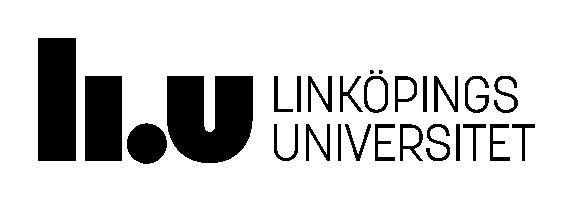
\includegraphics[width = 5cm]{liu_logga.png}

\vfill

{\normalsize
Division of Statistics and Machine Learning\\
Department of Computer and Information Science\\
Linköping University\\
\today\par}

\end{titlepage}

% \clearpage
% \thispagestyle{empty}
% \vspace*{\fill}
%
% \clearpage
% \setcounter{page}{1}
}
\makeatletter
\@ifpackageloaded{caption}{}{\usepackage{caption}}
\AtBeginDocument{%
\ifdefined\contentsname
  \renewcommand*\contentsname{Table of contents}
\else
  \newcommand\contentsname{Table of contents}
\fi
\ifdefined\listfigurename
  \renewcommand*\listfigurename{List of Figures}
\else
  \newcommand\listfigurename{List of Figures}
\fi
\ifdefined\listtablename
  \renewcommand*\listtablename{List of Tables}
\else
  \newcommand\listtablename{List of Tables}
\fi
\ifdefined\figurename
  \renewcommand*\figurename{Figure}
\else
  \newcommand\figurename{Figure}
\fi
\ifdefined\tablename
  \renewcommand*\tablename{Table}
\else
  \newcommand\tablename{Table}
\fi
}
\@ifpackageloaded{float}{}{\usepackage{float}}
\floatstyle{ruled}
\@ifundefined{c@chapter}{\newfloat{codelisting}{h}{lop}}{\newfloat{codelisting}{h}{lop}[chapter]}
\floatname{codelisting}{Listing}
\newcommand*\listoflistings{\listof{codelisting}{List of Listings}}
\makeatother
\makeatletter
\makeatother
\makeatletter
\@ifpackageloaded{caption}{}{\usepackage{caption}}
\@ifpackageloaded{subcaption}{}{\usepackage{subcaption}}
\makeatother

\ifLuaTeX
\usepackage[bidi=basic]{babel}
\else
\usepackage[bidi=default]{babel}
\fi
\babelprovide[main,import]{english}
% get rid of language-specific shorthands (see #6817):
\let\LanguageShortHands\languageshorthands
\def\languageshorthands#1{}
\ifLuaTeX
  \usepackage{selnolig}  % disable illegal ligatures
\fi
\usepackage{bookmark}

\IfFileExists{xurl.sty}{\usepackage{xurl}}{} % add URL line breaks if available
\urlstyle{same} % disable monospaced font for URLs
\hypersetup{
  pdflang={en},
  colorlinks=true,
  linkcolor={blue},
  filecolor={Maroon},
  citecolor={Blue},
  urlcolor={Blue},
  pdfcreator={LaTeX via pandoc}}


\author{}
\date{}

\begin{document}


\makereportfrontpage

\clearpage

\pagenumbering{arabic}
\setcounter{page}{1}

\justifying

\section{Assignment 1}\label{assignment-1}

\clearpage

\section{Assignment 2}\label{assignment-2}

\clearpage

\section{Assignment 3 - Logistic regression and Basis Function
Expansion}\label{assignment-3---logistic-regression-and-basis-function-expansion}

Visualization of the data shows that there are values equal to zero in
the measures, including plasma glucose which is one of the predictors of
interest in this assignment. \texttt{Glucose\ =\ 0} is not a feasible
value, but rather representing a missing value. All cases (n=5) with
plasma glucose equal to zero were excluded from the data before the
regression analysis.

\subsection{Scatterplot diabetes vs
age}\label{scatterplot-diabetes-vs-age}

\begin{figure}

\centering{

\includegraphics[width=0.6\textwidth,height=\textheight]{lab1_report_files/figure-pdf/fig-scatter-glucose-age-1.pdf}

}

\caption{\label{fig-scatter-glucose-age}Plasma glucose levels in
relation to age. Blue dots represent non-diabetic subjects, the pink
dots diabetic subjects.}

\end{figure}%

Plotting plasma glucose levels vs.~age shows that the two response
groups, \emph{Non-diabetic} and \emph{Diabetic}, show a substantial
overlap. \texttt{Diabetes} would therefore not be easily predicted by
\emph{Age} and \emph{Glucose} in a standard logistic regression model
which would not be able to derive a straight line clearly separating the
groups.

\subsection{Logistic regression model}\label{logistic-regression-model}

The vector form of the probailistic equation for a logistic regression
model is \begin{equation}\phantomsection\label{eq-logistic}{
P(Y = 1 \mid \mathit{x}) = \operatorname{sigmoid}(\boldsymbol{\theta}^{T}\mathit{x})
}\end{equation} where the sigmoid function is
\begin{equation}\phantomsection\label{eq-sigmoid}{
\mathit{sigmoid}(\boldsymbol{\theta}^{T}\mathit{x}) = \frac{1}{1 + e^{-\boldsymbol{\theta}^{T}\mathit{x}}}
}\end{equation}

For \emph{Diabetes} as the binary target/response (y), and
\emph{Glucose} and \emph{Age} as features/predictors (x1, x2):

\begin{equation}\phantomsection\label{eq-logistic-expanded}{
P(Y = 1 \mid x_1, x_2) = \frac{1}{1 + e^{-(\theta_0 + \theta_1 \cdot x_1 + \theta_2 \cdot x_2)}}
}\end{equation} Training a logistic regression model on the (entire)
provided data set, using glm() in R, results in the coefficients
\(\theta_0 = -6.2252\), \(\theta_1 = 0.0384\), and
\(\theta_2 = 0.0231\), all with significant p values, and the
corresponding probabilistic equation is then

\begin{equation}\phantomsection\label{eq-logistic-fitted}{
P(Y=1 \mid x_1,x_2) =
\frac{1}{1 + e^{-(
-6.2252 +
0.0384x_1 +
0.0231x_2)}}
}\end{equation}

The training misclassification error for this model (with r = 0.5) is
0.26, i.e approximately one out of four observations are misclassified.

\subsection{Scatterplot colored by
predicions}\label{scatterplot-colored-by-predicions}

\begin{figure}

\centering{

\includegraphics[width=0.6\textwidth,height=\textheight]{lab1_report_files/figure-pdf/fig-scatter-glucose-age-predictions-1.pdf}

}

\caption{\label{fig-scatter-glucose-age-predictions}Plasma glucose
levels in relation to age. Purple stars represent subjects predicted to
be non-diabetic, the orange stars subjects predicted to be diabetic.}

\end{figure}%

Comparing the predicted diabetes classifications to the actual diabetes
status as shown in Figure~\ref{fig-scatter-glucose-age} it looks like
there will be some misclassifications, possibly more so for subjects in
the lower, middle part of the scatter, where diabetic an non-diabetic
subjects are overlapping, and for the non-diabetic elderly subjects.

\subsection{Decision boundary
equation}\label{decision-boundary-equation}

Setting the probabilistic equation in Equation~\ref{eq-logistic-fitted}
equal to \texttt{r} (here \texttt{=\ 0.5}) results in this approximate
decision boundary equation, with the fitted coefficients and \emph{x1 =
Glucose} and \emph{x2 = Age} :

\begin{equation}\phantomsection\label{eq-dbeq}{
-6.2252 +
0.0384\cdot Glucose +
0.0231\cdot Age = 0
}\end{equation}

Solving this for \emph{Glucose} gives the approximate linear decision
boundary line

\begin{equation}\phantomsection\label{eq-dbeq-glucose-solved}{
\mathit{Glucose} = 161.97 -0.6\cdot Age
}\end{equation}

\clearpage

\subsection{Scatterplot with decision boundary line for r =
0.5}\label{scatterplot-with-decision-boundary-line-for-r-0.5}

\begin{figure}[H]

\centering{

\includegraphics[width=0.6\textwidth,height=\textheight]{lab1_report_files/figure-pdf/fig-scatter-glucose-age-predictions-r05-line-1.pdf}

}

\caption{\label{fig-scatter-glucose-age-predictions-r05-line}Predicted
diabetes classifications with threshold r = 0.5. The added black line is
the decision boundary line.}

\end{figure}%

The boundary line means that there will likely be misclassifications
both ways in the mixed ``middle'' group. The elderly non-diabetics will
risk being misclassified as diabetic according to the negative slope of
the linear boundary imposing increasingly harder restrictions on
acceptable plasma glucose level for a non-diabetic subject.

\subsection{Scatterplot with decision boundary line for r = 0.2 and r =
0.8}\label{scatterplot-with-decision-boundary-line-for-r-0.2-and-r-0.8}

The equation for the linear decision boundary line for two
predictors/features can generically be expressed as

\begin{equation}\phantomsection\label{eq-linear-boundary-generic}{
x_1 = \frac{\log\left(\frac{r}{1-r}\right) - \theta_0}{\theta_1} - \frac{\theta_2}{\theta_1}x_2
}\end{equation}

which means the intercept changes with r, the slope does not.

With r = 0.2 are more individuals predicted to be diabetic, with r
increased to 0.8 instead fewer individuals. The training
misclassification errors are 0.36 and 0.31 resepectively for the 0.2 and
0.8 cases, both higher than for the 0.5 cutoff case.

\begin{figure}

\centering{

\includegraphics{lab1_report_files/figure-pdf/fig-diabetes-thresholds-pw-1.pdf}

}

\caption{\label{fig-diabetes-thresholds-pw}Predicted diabetes
classifications for thresholds r = 0.2 (left) and r = 0.8 (right). Black
lines indicate the decision boundaries.}

\end{figure}%

\subsection{Basis function expansion}\label{basis-function-expansion}

Fitting a new logistic regression model after adding new features

\[
z_1 = x_1^4, \quad
z_2 = x_1^3 x_2, \quad
z_3 = x_1^2 x_2^2, \quad
z_4 = x_1 x_2^3, \quad
z_5 = x_2^4
\] results in a much more complex model but a training misclassification
error (with r = 0.5) of 0.24 which is slightly better than the linear
model. The decision boundary is now not linear but curvilinear, changing
the appearance of the Glucose vs Age scatterplot (see
Figure~\ref{fig-extended-scatter}). The most obvious difference from the
previous model is that older subjects are ``allowed'' to have higher
plasma glucose levels without being predicted to be diabetic, which is a
pattern that can be discerned also in the actual data.

The \emph{theta3} to \emph{theta7} coefficients (for the \emph{z1} to
\emph{z5} terms) are very small (magnitude \$10\^{}\{-7\} or less), and
individually non-significant (p values above 0.6), but they are
multiplied with numerically high values for \emph{Glucose} (raised to up
to 4) in the polynomial, and the AIC reduction suggests an improved
overall fit for the model.

\begin{figure}[H]

\centering{

\includegraphics[width=0.6\textwidth,height=\textheight]{lab1_report_files/figure-pdf/fig-extended-scatter-1.pdf}

}

\caption{\label{fig-extended-scatter}Predicted diabetes classifications
for the extended logistic regression model with polynomial basis
function expansion.}

\end{figure}%

\clearpage

\section{Theory}\label{theory}

\clearpage

\clearpage

\appendix

\section{R code}\label{r-code}

\subsection{Assignment 1}\label{assignment-1-1}

\subsection{Assignment 2}\label{assignment-2-1}

\subsection{Assignment 3}\label{assignment-3}

\subsubsection{Assignment 3 --- Functions}\label{assignment-3-functions}

\begin{Shaded}
\begin{Highlighting}[]
\DocumentationTok{\#\#\#\#\#\#\#\#\#\#\#\#\#\#\#\#\#\#\#\#\#\#\#\#\#\#\#\#\#\#\#\#\#\#\#\#\#\#\#\#\#\#\#\#\#\#\#\#\#\#\#\#\#\#\#\#\#\#\#\#\#\#\#\#\#\#\#\#\#\#\#\#\#\#\#\#\#\#\#\#}
\CommentTok{\# function definitions}

\DocumentationTok{\#\#\#\#\#\#\#\#\#\#\#\#\#\#\#\#\#\#\#\#\#\#\#\#\#\#\#\#\#\#\#\#\#\#\#\#\#\#\#\#\#\#\#\#\#\#\#\#\#\#\#\#\#\#\#\#\#\#\#\#\#\#\#\#\#\#\#\#\#\#\#\#\#\#\#\#\#\#\#\#}
\CommentTok{\#\textquotesingle{} A3\_classifications\_and\_plots}
\CommentTok{\#\textquotesingle{} Adds predictions based on provided predicted probabilities}
\CommentTok{\#\textquotesingle{} and decision threshold, and creates a plot colored by diabetes prediction}
\CommentTok{\#\textquotesingle{} and a plot colored by the predicion being correct or not,}
\CommentTok{\#\textquotesingle{} the latter is extra so not presented in report.}
\CommentTok{\#\textquotesingle{}}
\CommentTok{\#\textquotesingle{} @param data\_pred\_prob A tibble with data and predicted probabilities}
\CommentTok{\#\textquotesingle{} @param r Classification threshold}
\CommentTok{\#\textquotesingle{} @param glucose\_range Numerical vector with min and max of Glucose values}
\CommentTok{\#\textquotesingle{} @param age\_range Numerical vector with min and max of Age values}
\CommentTok{\#\textquotesingle{}}
\CommentTok{\#\textquotesingle{} @returns A list of:}
\CommentTok{\#\textquotesingle{} data\_with\_predictions}
\CommentTok{\#\textquotesingle{}    = data where Diabetes\_prediction and Correct\_prediction}
\CommentTok{\#\textquotesingle{}    columns (both logical) are added}
\CommentTok{\#\textquotesingle{} confusion\_matrix}
\CommentTok{\#\textquotesingle{}    = confusion matrix for Actual vs Predicted diabetes}
\CommentTok{\#\textquotesingle{} correct\_proportion}
\CommentTok{\#\textquotesingle{}    = Proportion of correctly classified observations}
\CommentTok{\#\textquotesingle{} training\_misclass\_error}
\CommentTok{\#\textquotesingle{}    = Proportion of misclassified observations}
\CommentTok{\#\textquotesingle{} pred\_plot}
\CommentTok{\#\textquotesingle{}    = Plot of Glucose vs Age, colored by Diabetes\_predicion}
\CommentTok{\#\textquotesingle{} class\_plot}
\CommentTok{\#\textquotesingle{}    = Plot of Glucose vs Age, colored by Correct\_pred}
\CommentTok{\#\textquotesingle{}}
\NormalTok{A3\_classifications\_and\_plots }\OtherTok{\textless{}{-}}
  \ControlFlowTok{function}\NormalTok{(data\_pred\_prob, r, glucose\_range, age\_range)\{}

  \CommentTok{\# adding prediction classifications to the data tibble}
\NormalTok{  data\_with\_predictions }\OtherTok{\textless{}{-}}
\NormalTok{    data\_pred\_prob }\SpecialCharTok{|\textgreater{}}
    \FunctionTok{mutate}\NormalTok{(}\AttributeTok{Diabetes\_prediction =} \FunctionTok{ifelse}\NormalTok{(Predicted\_prob }\SpecialCharTok{\textgreater{}}\NormalTok{ r, }\ConstantTok{TRUE}\NormalTok{, }\ConstantTok{FALSE}\NormalTok{),}
           \AttributeTok{Correct\_pred =}\NormalTok{ (Diabetes }\SpecialCharTok{==}\NormalTok{ Diabetes\_prediction))}

  \CommentTok{\# confusion matrix}
\NormalTok{  logistic\_confusion }\OtherTok{\textless{}{-}}
    \FunctionTok{table}\NormalTok{(}\AttributeTok{Actual =}\NormalTok{ data\_with\_predictions}\SpecialCharTok{$}\NormalTok{Diabetes,}
          \AttributeTok{Predicted =}\NormalTok{ data\_with\_predictions}\SpecialCharTok{$}\NormalTok{Diabetes\_prediction)}

  \CommentTok{\# proportion correctly classified observations}
\NormalTok{  correct\_proportion }\OtherTok{\textless{}{-}}
    \FunctionTok{sum}\NormalTok{(}\FunctionTok{diag}\NormalTok{(logistic\_confusion))}\SpecialCharTok{/}\FunctionTok{sum}\NormalTok{(logistic\_confusion)}

  \CommentTok{\# training misclassification error}
  \CommentTok{\# = proportion of misclassified observations}
\NormalTok{  training\_misclass\_error }\OtherTok{\textless{}{-}}
    \DecValTok{1} \SpecialCharTok{{-}}\NormalTok{ correct\_proportion}

  \CommentTok{\# scatterplot colored by predictions}
\NormalTok{  pred\_plot }\OtherTok{\textless{}{-}}
\NormalTok{    data\_with\_predictions }\SpecialCharTok{|\textgreater{}}
    \FunctionTok{ggplot}\NormalTok{() }\SpecialCharTok{+}
    \FunctionTok{aes}\NormalTok{(}\AttributeTok{x =}\NormalTok{ Age, }\AttributeTok{y =}\NormalTok{ Glucose, }\AttributeTok{color =}\NormalTok{ Diabetes\_prediction) }\SpecialCharTok{+}
    \FunctionTok{geom\_point}\NormalTok{(}\AttributeTok{size =} \FloatTok{0.3}\NormalTok{, }\AttributeTok{shape =} \DecValTok{8}\NormalTok{) }\SpecialCharTok{+}
    \FunctionTok{theme\_bw}\NormalTok{() }\SpecialCharTok{+}
    \FunctionTok{theme\_bw}\NormalTok{() }\SpecialCharTok{+}
    \FunctionTok{theme}\NormalTok{(}\AttributeTok{legend.position =} \StringTok{"top"}\NormalTok{) }\SpecialCharTok{+}
    \FunctionTok{scale\_colour\_manual}\NormalTok{(}\AttributeTok{labels =} \FunctionTok{c}\NormalTok{(}\StringTok{"Non{-}diabetic"}\NormalTok{, }\StringTok{"Diabetic"}\NormalTok{),}
                        \AttributeTok{values =} \FunctionTok{c}\NormalTok{(}\StringTok{"darkmagenta"}\NormalTok{, }\StringTok{"darkorange"}\NormalTok{)) }\SpecialCharTok{+}
    \FunctionTok{scale\_x\_continuous}\NormalTok{(}
      \AttributeTok{limits =}\NormalTok{ age\_range }\SpecialCharTok{+} \FunctionTok{c}\NormalTok{(}\SpecialCharTok{{-}}\DecValTok{5}\NormalTok{, }\SpecialCharTok{+}\DecValTok{5}\NormalTok{),}
      \AttributeTok{breaks =}\NormalTok{ scales}\SpecialCharTok{::}\FunctionTok{breaks\_width}\NormalTok{(}\DecValTok{10}\NormalTok{)) }\SpecialCharTok{+}
    \FunctionTok{scale\_y\_continuous}\NormalTok{(}
      \AttributeTok{limits =}\NormalTok{ glucose\_range }\SpecialCharTok{+} \FunctionTok{c}\NormalTok{(}\SpecialCharTok{{-}}\DecValTok{5}\NormalTok{, }\SpecialCharTok{+}\DecValTok{5}\NormalTok{),}
      \AttributeTok{breaks =}\NormalTok{ scales}\SpecialCharTok{::}\FunctionTok{breaks\_width}\NormalTok{(}\DecValTok{10}\NormalTok{),}
      \AttributeTok{expand =} \FunctionTok{expansion}\NormalTok{(}\AttributeTok{mult =} \FunctionTok{c}\NormalTok{(}\DecValTok{0}\NormalTok{, }\FloatTok{0.05}\NormalTok{))}
\NormalTok{    ) }\SpecialCharTok{+}
    \FunctionTok{labs}\NormalTok{(}\AttributeTok{y =} \StringTok{"Plasma glucose"}\NormalTok{, }\AttributeTok{color =} \StringTok{"Diabetes prediction"}\NormalTok{)}

  \CommentTok{\# scatterplot colored by correct or misclassfication}
\NormalTok{  class\_plot }\OtherTok{\textless{}{-}}
\NormalTok{    data\_with\_predictions }\SpecialCharTok{|\textgreater{}}
    \FunctionTok{ggplot}\NormalTok{() }\SpecialCharTok{+}
    \FunctionTok{aes}\NormalTok{(}\AttributeTok{x =}\NormalTok{ Age, }\AttributeTok{y =}\NormalTok{ Glucose, }\AttributeTok{color =}\NormalTok{ Correct\_pred, }\AttributeTok{shape =}\NormalTok{ Correct\_pred) }\SpecialCharTok{+}
    \FunctionTok{geom\_point}\NormalTok{(}\AttributeTok{size =} \FloatTok{0.3}\NormalTok{) }\SpecialCharTok{+}
    \FunctionTok{theme\_bw}\NormalTok{() }\SpecialCharTok{+}
    \FunctionTok{theme}\NormalTok{(}\AttributeTok{legend.position =} \StringTok{"top"}\NormalTok{) }\SpecialCharTok{+}
    \FunctionTok{scale\_colour\_manual}\NormalTok{(}
      \AttributeTok{name =} \StringTok{"Classification result"}\NormalTok{,}
      \AttributeTok{values =} \FunctionTok{c}\NormalTok{(}\StringTok{\textasciigrave{}}\AttributeTok{TRUE}\StringTok{\textasciigrave{}} \OtherTok{=} \StringTok{"green"}\NormalTok{, }\StringTok{\textasciigrave{}}\AttributeTok{FALSE}\StringTok{\textasciigrave{}} \OtherTok{=} \StringTok{"red"}\NormalTok{),}
      \AttributeTok{labels =} \FunctionTok{c}\NormalTok{(}\StringTok{\textasciigrave{}}\AttributeTok{TRUE}\StringTok{\textasciigrave{}} \OtherTok{=} \StringTok{"Correct"}\NormalTok{, }\StringTok{\textasciigrave{}}\AttributeTok{FALSE}\StringTok{\textasciigrave{}} \OtherTok{=} \StringTok{"Misclassification"}\NormalTok{)}
\NormalTok{    ) }\SpecialCharTok{+}
    \FunctionTok{scale\_shape\_manual}\NormalTok{(}
      \AttributeTok{name =} \StringTok{"Classification result"}\NormalTok{,}
      \AttributeTok{values =} \FunctionTok{c}\NormalTok{(}\StringTok{\textasciigrave{}}\AttributeTok{TRUE}\StringTok{\textasciigrave{}} \OtherTok{=} \DecValTok{18}\NormalTok{, }\StringTok{\textasciigrave{}}\AttributeTok{FALSE}\StringTok{\textasciigrave{}} \OtherTok{=} \DecValTok{4}\NormalTok{),}
      \AttributeTok{labels =} \FunctionTok{c}\NormalTok{(}\StringTok{\textasciigrave{}}\AttributeTok{TRUE}\StringTok{\textasciigrave{}} \OtherTok{=} \StringTok{"Correct"}\NormalTok{, }\StringTok{\textasciigrave{}}\AttributeTok{FALSE}\StringTok{\textasciigrave{}} \OtherTok{=} \StringTok{"Misclassification"}\NormalTok{)}
\NormalTok{    ) }\SpecialCharTok{+}
    \FunctionTok{scale\_x\_continuous}\NormalTok{(}
      \AttributeTok{limits =}\NormalTok{ age\_range }\SpecialCharTok{+} \FunctionTok{c}\NormalTok{(}\SpecialCharTok{{-}}\DecValTok{5}\NormalTok{, }\SpecialCharTok{+}\DecValTok{5}\NormalTok{),}
      \AttributeTok{breaks =}\NormalTok{ scales}\SpecialCharTok{::}\FunctionTok{breaks\_width}\NormalTok{(}\DecValTok{10}\NormalTok{)) }\SpecialCharTok{+}
    \FunctionTok{scale\_y\_continuous}\NormalTok{(}
      \AttributeTok{limits =}\NormalTok{ glucose\_range }\SpecialCharTok{+} \FunctionTok{c}\NormalTok{(}\SpecialCharTok{{-}}\DecValTok{5}\NormalTok{, }\SpecialCharTok{+}\DecValTok{5}\NormalTok{),}
      \AttributeTok{breaks =}\NormalTok{ scales}\SpecialCharTok{::}\FunctionTok{breaks\_width}\NormalTok{(}\DecValTok{10}\NormalTok{),}
      \AttributeTok{expand =} \FunctionTok{expansion}\NormalTok{(}\AttributeTok{mult =} \FunctionTok{c}\NormalTok{(}\DecValTok{0}\NormalTok{, }\FloatTok{0.05}\NormalTok{))}
\NormalTok{    )}

  \FunctionTok{return}\NormalTok{(}\FunctionTok{list}\NormalTok{(}\AttributeTok{data\_with\_predictions =}\NormalTok{ data\_with\_predictions,}
              \AttributeTok{confusion\_matrix =}\NormalTok{ logistic\_confusion,}
              \AttributeTok{correct\_proportion =}\NormalTok{ correct\_proportion,}
              \AttributeTok{training\_misclass\_error =}\NormalTok{ training\_misclass\_error,}
              \AttributeTok{pred\_plot =}\NormalTok{ pred\_plot,}
              \AttributeTok{class\_plot =}\NormalTok{ class\_plot))}
\NormalTok{\}}

\DocumentationTok{\#\#\#\#\#\#\#\#\#\#\#\#\#\#\#\#\#\#\#\#\#\#\#\#\#\#\#\#\#\#\#\#\#\#\#\#\#\#\#\#\#\#\#\#\#\#\#\#\#\#\#\#\#\#\#\#\#\#\#\#\#\#\#\#\#\#\#\#\#\#\#\#\#\#\#\#\#\#\#\#}
\CommentTok{\#\textquotesingle{} A3\_calculate\_linear\_boundary}
\CommentTok{\#\textquotesingle{} Calculating a linear boundary intercept and slope}
\CommentTok{\#\textquotesingle{}}
\CommentTok{\#\textquotesingle{} @param theta0 Fitted intercept}
\CommentTok{\#\textquotesingle{} @param theta1 Fitted coefficient for Glucose}
\CommentTok{\#\textquotesingle{} @param theta2 Fitted coefficient for Age}
\CommentTok{\#\textquotesingle{}}
\CommentTok{\#\textquotesingle{} @returns A list with boundary intercept and slope}
\CommentTok{\#\textquotesingle{}}
\NormalTok{A3\_calculate\_linear\_boundary }\OtherTok{\textless{}{-}} \ControlFlowTok{function}\NormalTok{(theta0, theta1, theta2, r)\{}

  \CommentTok{\# decision boundary line intercept and slope}
\NormalTok{  boundary\_intercept }\OtherTok{\textless{}{-}}\NormalTok{  (}\FunctionTok{log}\NormalTok{(r}\SpecialCharTok{/}\NormalTok{(}\DecValTok{1}\SpecialCharTok{{-}}\NormalTok{r))}\SpecialCharTok{{-}}\NormalTok{theta0)}\SpecialCharTok{/}\NormalTok{theta1}
\NormalTok{  boundary\_slope }\OtherTok{\textless{}{-}}  \SpecialCharTok{{-}}\NormalTok{theta2}\SpecialCharTok{/}\NormalTok{theta1}

  \FunctionTok{return}\NormalTok{(}\FunctionTok{list}\NormalTok{(}\AttributeTok{boundary\_intercept =}\NormalTok{ boundary\_intercept,}
              \AttributeTok{boundary\_slope =}\NormalTok{  boundary\_slope))}
\NormalTok{\}}

\DocumentationTok{\#\#\#\#\#\#\#\#\#\#\#\#\#\#\#\#\#\#\#\#\#\#\#\#\#\#\#\#\#\#\#\#\#\#\#\#\#\#\#\#\#\#\#\#\#\#\#\#\#\#\#\#\#\#\#\#\#\#\#\#\#\#\#\#\#\#\#\#\#\#\#\#\#\#\#\#\#\#\#\#}
\CommentTok{\#\textquotesingle{} A3\_add\_linear\_boundary}
\CommentTok{\#\textquotesingle{} Adds a decision boundary line to the provided plots}
\CommentTok{\#\textquotesingle{}}
\CommentTok{\#\textquotesingle{} @param results\_list List returned by}
\CommentTok{\#\textquotesingle{} A3\_classifications\_and\_plots}
\CommentTok{\#\textquotesingle{}}
\CommentTok{\#\textquotesingle{} @returns A list of two plots,}
\CommentTok{\#\textquotesingle{} one colored by diabetes prediction, and}
\CommentTok{\#\textquotesingle{} one colored by the predicion being correct or not}
\CommentTok{\#\textquotesingle{}}
\NormalTok{A3\_add\_linear\_boundary }\OtherTok{\textless{}{-}}  \ControlFlowTok{function}\NormalTok{(results\_list, r )\{}
  \CommentTok{\# calculate intercept and slope for the straight line}
\NormalTok{  boundary }\OtherTok{\textless{}{-}}
    \FunctionTok{A3\_calculate\_linear\_boundary}\NormalTok{(A3\_theta0, A3\_theta1, A3\_theta2, r)}

  \CommentTok{\# add line to prediction plot}
\NormalTok{  pred\_plot\_with\_line }\OtherTok{\textless{}{-}}
\NormalTok{    results\_list[[}\StringTok{"pred\_plot"}\NormalTok{]] }\SpecialCharTok{+}
    \FunctionTok{geom\_abline}\NormalTok{(}
      \AttributeTok{intercept =}\NormalTok{ boundary[[}\StringTok{"boundary\_intercept"}\NormalTok{]],}
      \AttributeTok{slope =}\NormalTok{ boundary[[}\StringTok{"boundary\_slope"}\NormalTok{]],}
      \AttributeTok{color =} \StringTok{"black"}\NormalTok{,}
      \AttributeTok{linewidth =} \DecValTok{1}
\NormalTok{    )}

  \CommentTok{\# add line to classification correctness plot}
\NormalTok{  class\_plot\_with\_line }\OtherTok{\textless{}{-}}
\NormalTok{    results\_list[[}\StringTok{"class\_plot"}\NormalTok{]] }\SpecialCharTok{+}
    \FunctionTok{geom\_abline}\NormalTok{(}
      \AttributeTok{intercept =}\NormalTok{ boundary[[}\StringTok{"boundary\_intercept"}\NormalTok{]],}
      \AttributeTok{slope =}\NormalTok{ boundary[[}\StringTok{"boundary\_slope"}\NormalTok{]],}
      \AttributeTok{color =} \StringTok{"black"}\NormalTok{,}
      \AttributeTok{linewidth =} \DecValTok{1}
\NormalTok{    )}
  \FunctionTok{return}\NormalTok{(}\FunctionTok{list}\NormalTok{(}\AttributeTok{pred\_plot\_with\_line=}\NormalTok{pred\_plot\_with\_line,}
              \AttributeTok{class\_plot\_with\_line=}\NormalTok{class\_plot\_with\_line))}
\NormalTok{\}}

\DocumentationTok{\#\#\#\#\#\#\#\#\#\#\#\#\#\#\#\#\#\#\#\#\#\#\#\#\#\#\#\#\#\#\#\#\#\#\#\#\#\#\#\#\#\#\#\#\#\#\#\#\#\#\#\#\#\#\#\#\#\#\#\#\#\#\#\#\#\#\#\#\#\#\#\#\#\#\#\#\#\#\#\#}
\end{Highlighting}
\end{Shaded}

\subsubsection{Assignment 3 --- Main
script}\label{assignment-3-main-script}

\begin{Shaded}
\begin{Highlighting}[]
\FunctionTok{library}\NormalTok{(tidyverse)}

\CommentTok{\# Data in pima{-}indians{-}diabetes.csv:}
\CommentTok{\# 1. Number of times pregnant.}
\CommentTok{\# 2. Plasma glucose concentration at 2 hours in an oral glucose tolerance test.}
\CommentTok{\# 3. Diastolic blood pressure (mm Hg).}
\CommentTok{\# 4. Triceps skinfold thickness (mm).}
\CommentTok{\# 5. 2{-}Hour serum insulin (mu U/ml).}
\CommentTok{\# 6. Body mass index (weight in kg/(height in m)\^{}2).}
\CommentTok{\# 7. Diabetes pedigree function.}
\CommentTok{\# 8. Age (years).}
\CommentTok{\# 9. Diabetes (0=no or 1=yes).}

\CommentTok{\# import user{-}definied functions}
\FunctionTok{source}\NormalTok{(}\StringTok{"R/lab1\_assignment3\_functions.R"}\NormalTok{)}

\CommentTok{\# read data}
\NormalTok{A3\_pimadata }\OtherTok{\textless{}{-}} \FunctionTok{read.csv}\NormalTok{(}\StringTok{"data/pima{-}indians{-}diabetes.csv"}\NormalTok{)}

\CommentTok{\# any NA:s?}
\ControlFlowTok{if}\NormalTok{ (}\FunctionTok{anyNA}\NormalTok{(A3\_pimadata)) \{}
  \FunctionTok{message}\NormalTok{(}\StringTok{"NA:s in table"}\NormalTok{)}
\NormalTok{\}}

\CommentTok{\# create tibble with meaningful column names}
\NormalTok{A3\_pimatibble\_raw }\OtherTok{\textless{}{-}}
\NormalTok{  A3\_pimadata }\SpecialCharTok{|\textgreater{}}
  \FunctionTok{tibble}\NormalTok{() }\SpecialCharTok{|\textgreater{}}
\NormalTok{  magrittr}\SpecialCharTok{::}\FunctionTok{set\_colnames}\NormalTok{(}\FunctionTok{c}\NormalTok{(}\StringTok{"Parity"}\NormalTok{, }\StringTok{"Glucose"}\NormalTok{, }\StringTok{"DBP"}\NormalTok{, }\StringTok{"Skinfold"}\NormalTok{,}
                           \StringTok{"Insulin"}\NormalTok{,}\StringTok{"BMI"}\NormalTok{, }\StringTok{"Pedigree"}\NormalTok{, }\StringTok{"Age"}\NormalTok{, }\StringTok{"Diabetes"}\NormalTok{)) }\SpecialCharTok{|\textgreater{}}
  \FunctionTok{mutate}\NormalTok{(}\AttributeTok{Diabetes =} \FunctionTok{as.logical}\NormalTok{(Diabetes)) }\SpecialCharTok{|\textgreater{}}
  \FunctionTok{mutate}\NormalTok{(}\AttributeTok{ID =} \FunctionTok{row\_number}\NormalTok{(), }\AttributeTok{.before =}\NormalTok{ Parity) }\SpecialCharTok{|\textgreater{}}
  \FunctionTok{select}\NormalTok{(ID, Age, Pedigree, Parity, BMI, Skinfold,}
\NormalTok{         DBP, Insulin, Glucose, Diabetes)}

\CommentTok{\# data check}
\NormalTok{  A3\_pimatibble\_raw }\SpecialCharTok{|\textgreater{}}
  \FunctionTok{pivot\_longer}\NormalTok{(}\SpecialCharTok{{-}}\FunctionTok{c}\NormalTok{(ID,Diabetes),}
               \AttributeTok{names\_to =} \StringTok{"Measure"}\NormalTok{,}
               \AttributeTok{values\_to =} \StringTok{"Value"}\NormalTok{) }\SpecialCharTok{|\textgreater{}}
  \FunctionTok{ggplot}\NormalTok{() }\SpecialCharTok{+}
  \FunctionTok{aes}\NormalTok{(}\AttributeTok{x=}\NormalTok{Value, }\AttributeTok{fill =}\NormalTok{ Diabetes) }\SpecialCharTok{+}
  \FunctionTok{geom\_histogram}\NormalTok{(}\AttributeTok{bins =} \DecValTok{30}\NormalTok{) }\SpecialCharTok{+}
  \FunctionTok{scale\_fill\_manual}\NormalTok{(}\AttributeTok{labels =} \FunctionTok{c}\NormalTok{(}\StringTok{"Non{-}diabetic"}\NormalTok{, }\StringTok{"Diabetic"}\NormalTok{),}
                      \AttributeTok{values =} \FunctionTok{c}\NormalTok{(}\StringTok{"royalblue"}\NormalTok{, }\StringTok{"maroon2"}\NormalTok{)) }\SpecialCharTok{+}
  \FunctionTok{facet\_wrap}\NormalTok{(}\SpecialCharTok{\textasciitilde{}}\NormalTok{ Measure, }\AttributeTok{scales =} \StringTok{"free"}\NormalTok{, }\AttributeTok{nrow =} \DecValTok{2}\NormalTok{) }\SpecialCharTok{+}
  \FunctionTok{theme\_bw}\NormalTok{() }\SpecialCharTok{+}
  \FunctionTok{theme}\NormalTok{(}\AttributeTok{legend.position =} \StringTok{"top"}\NormalTok{)}

\CommentTok{\# checking exact range for Age, Glucose, and Diabetes}
\NormalTok{A3\_pimatibble\_raw }\SpecialCharTok{|\textgreater{}}
  \FunctionTok{select}\NormalTok{(}\FunctionTok{c}\NormalTok{(Age, Glucose, Diabetes)) }\SpecialCharTok{|\textgreater{}}
  \FunctionTok{map}\NormalTok{(\textbackslash{}(x) }\FunctionTok{range}\NormalTok{(x))}

\CommentTok{\# removing cases with Glucose = 0}
\NormalTok{A3\_pimatibble }\OtherTok{\textless{}{-}}
\NormalTok{  A3\_pimatibble\_raw }\SpecialCharTok{|\textgreater{}}
  \FunctionTok{filter}\NormalTok{(Glucose }\SpecialCharTok{!=} \DecValTok{0}\NormalTok{)}

\CommentTok{\# saving adjusted ranges}
\NormalTok{A3\_minmaxlist }\OtherTok{\textless{}{-}}
\NormalTok{  A3\_pimatibble }\SpecialCharTok{|\textgreater{}}
  \FunctionTok{select}\NormalTok{(Age, Glucose) }\SpecialCharTok{|\textgreater{}}
  \FunctionTok{map}\NormalTok{(\textbackslash{}(x) }\FunctionTok{tibble}\NormalTok{(}\AttributeTok{min =} \FunctionTok{min}\NormalTok{(x), }\AttributeTok{max =} \FunctionTok{max}\NormalTok{(x)))}

\NormalTok{A3\_Age\_range }\OtherTok{\textless{}{-}} \FunctionTok{unlist}\NormalTok{(A3\_minmaxlist[[}\StringTok{"Age"}\NormalTok{]])}
\NormalTok{A3\_Glucose\_range }\OtherTok{\textless{}{-}} \FunctionTok{unlist}\NormalTok{(A3\_minmaxlist[[}\StringTok{"Glucose"}\NormalTok{]], }\AttributeTok{use.names =} \ConstantTok{FALSE}\NormalTok{)}

\CommentTok{\# scatterplot Glucose vs Age}

\NormalTok{A3\_Glucose\_vs\_Age\_scatter }\OtherTok{\textless{}{-}}
\NormalTok{  A3\_pimatibble }\SpecialCharTok{|\textgreater{}}
  \FunctionTok{ggplot}\NormalTok{() }\SpecialCharTok{+}
  \FunctionTok{aes}\NormalTok{(}\AttributeTok{x =}\NormalTok{ Age, }\AttributeTok{y =}\NormalTok{ Glucose, }\AttributeTok{color =}\NormalTok{ Diabetes) }\SpecialCharTok{+}
  \FunctionTok{geom\_point}\NormalTok{(}\AttributeTok{size =} \FloatTok{0.5}\NormalTok{, }\AttributeTok{alpha =} \FloatTok{0.8}\NormalTok{) }\SpecialCharTok{+}
  \FunctionTok{theme\_bw}\NormalTok{() }\SpecialCharTok{+}
  \FunctionTok{theme}\NormalTok{(}\AttributeTok{legend.position =} \StringTok{"top"}\NormalTok{) }\SpecialCharTok{+}
  \FunctionTok{scale\_colour\_manual}\NormalTok{(}\AttributeTok{labels =} \FunctionTok{c}\NormalTok{(}\StringTok{"Non{-}diabetic"}\NormalTok{, }\StringTok{"Diabetic"}\NormalTok{),}
                      \AttributeTok{values =} \FunctionTok{c}\NormalTok{(}\StringTok{"royalblue"}\NormalTok{, }\StringTok{"maroon2"}\NormalTok{)) }\SpecialCharTok{+}
  \FunctionTok{scale\_x\_continuous}\NormalTok{(}
    \AttributeTok{limits =}\NormalTok{ A3\_Age\_range }\SpecialCharTok{+} \FunctionTok{c}\NormalTok{(}\SpecialCharTok{{-}}\DecValTok{5}\NormalTok{, }\SpecialCharTok{+}\DecValTok{5}\NormalTok{),}
    \AttributeTok{breaks =}\NormalTok{ scales}\SpecialCharTok{::}\FunctionTok{breaks\_width}\NormalTok{(}\AttributeTok{width=}\DecValTok{10}\NormalTok{)) }\SpecialCharTok{+} \CommentTok{\# equally spaced breaks}
  \FunctionTok{scale\_y\_continuous}\NormalTok{(}
    \AttributeTok{limits =}\NormalTok{ A3\_Glucose\_range }\SpecialCharTok{+} \FunctionTok{c}\NormalTok{(}\SpecialCharTok{{-}}\DecValTok{5}\NormalTok{, }\SpecialCharTok{+}\DecValTok{5}\NormalTok{),}
    \AttributeTok{breaks =}\NormalTok{ scales}\SpecialCharTok{::}\FunctionTok{breaks\_width}\NormalTok{(}\DecValTok{10}\NormalTok{),}
    \AttributeTok{expand =} \FunctionTok{expansion}\NormalTok{(}\AttributeTok{mult =} \FunctionTok{c}\NormalTok{(}\DecValTok{0}\NormalTok{, }\FloatTok{0.05}\NormalTok{))}
\NormalTok{  ) }\SpecialCharTok{+}
  \FunctionTok{labs}\NormalTok{(}\AttributeTok{y =} \StringTok{"Plasma glucose"}\NormalTok{)}

\CommentTok{\# training a logistic regression model}

\CommentTok{\# Diabetes \textasciitilde{} Glucose + Age in a logistic regression model}
\CommentTok{\# using glm()= with family = "binomial" since target has two levels}

\NormalTok{A3\_logistic\_model }\OtherTok{\textless{}{-}}
  \FunctionTok{glm}\NormalTok{(Diabetes }\SpecialCharTok{\textasciitilde{}}\NormalTok{ Glucose }\SpecialCharTok{+}\NormalTok{ Age, }\AttributeTok{data =}\NormalTok{ A3\_pimatibble, }\AttributeTok{family =} \StringTok{"binomial"}\NormalTok{)}

\FunctionTok{summary}\NormalTok{(A3\_logistic\_model)}

\CommentTok{\# coefficients (= coefficients in the probabilistic equation)}

\NormalTok{A3\_logistic\_coef }\OtherTok{\textless{}{-}} \FunctionTok{coef}\NormalTok{(A3\_logistic\_model)}

\NormalTok{A3\_theta0 }\OtherTok{\textless{}{-}}\NormalTok{ A3\_logistic\_coef[}\StringTok{"(Intercept)"}\NormalTok{]}
\NormalTok{A3\_theta1 }\OtherTok{\textless{}{-}}\NormalTok{ A3\_logistic\_coef[}\StringTok{"Glucose"}\NormalTok{]}
\NormalTok{A3\_theta2 }\OtherTok{\textless{}{-}}\NormalTok{ A3\_logistic\_coef[}\StringTok{"Age"}\NormalTok{]}

\CommentTok{\# adding predicted probabilities to data}
\NormalTok{A3\_pimatibble\_pred\_probs }\OtherTok{\textless{}{-}}
\NormalTok{  A3\_pimatibble }\SpecialCharTok{|\textgreater{}}
  \FunctionTok{mutate}\NormalTok{(}\AttributeTok{Predicted\_prob =} \FunctionTok{predict}\NormalTok{(A3\_logistic\_model, }\AttributeTok{type =} \StringTok{"response"}\NormalTok{))}

\CommentTok{\# adding predicted diabetess classification}
\CommentTok{\# and comparison with actual diabetes class}
\CommentTok{\# and plot visualizing the results}
\NormalTok{A3\_results\_r\_05 }\OtherTok{\textless{}{-}}
  \FunctionTok{A3\_classifications\_and\_plots}\NormalTok{(A3\_pimatibble\_pred\_probs,}
                               \AttributeTok{r =} \FloatTok{0.5}\NormalTok{, A3\_Glucose\_range, A3\_Age\_range)}

\NormalTok{A3\_results\_r\_02 }\OtherTok{\textless{}{-}}
  \FunctionTok{A3\_classifications\_and\_plots}\NormalTok{(A3\_pimatibble\_pred\_probs,}
                               \AttributeTok{r =} \FloatTok{0.2}\NormalTok{, A3\_Glucose\_range, A3\_Age\_range)}

\NormalTok{A3\_results\_r\_08 }\OtherTok{\textless{}{-}}
  \FunctionTok{A3\_classifications\_and\_plots}\NormalTok{(A3\_pimatibble\_pred\_probs,}
                            \AttributeTok{r =} \FloatTok{0.8}\NormalTok{, A3\_Glucose\_range, A3\_Age\_range)}

\CommentTok{\# adding decision boundary lines to Glucose vs Age plots}
\NormalTok{A3\_boundary\_05\_plots }\OtherTok{\textless{}{-}}
  \FunctionTok{A3\_add\_linear\_boundary}\NormalTok{(A3\_results\_r\_05, }\AttributeTok{r =} \FloatTok{0.5}\NormalTok{)}

\NormalTok{A3\_boundary\_02\_plots }\OtherTok{\textless{}{-}}
  \FunctionTok{A3\_add\_linear\_boundary}\NormalTok{(A3\_results\_r\_02, }\AttributeTok{r =} \FloatTok{0.2}\NormalTok{)}

\NormalTok{A3\_boundary\_08\_plots }\OtherTok{\textless{}{-}}
  \FunctionTok{A3\_add\_linear\_boundary}\NormalTok{(A3\_results\_r\_08, }\AttributeTok{r =} \FloatTok{0.8}\NormalTok{)}

\CommentTok{\# basis function expansion}
\CommentTok{\# sdding new features}
\NormalTok{A3\_pimatibble\_extended }\OtherTok{\textless{}{-}}
\NormalTok{  A3\_pimatibble }\SpecialCharTok{|\textgreater{}}
  \FunctionTok{mutate}\NormalTok{(}\AttributeTok{z1 =}\NormalTok{ Glucose}\SpecialCharTok{\^{}}\DecValTok{4}\NormalTok{,}
         \AttributeTok{z2 =}\NormalTok{ Glucose}\SpecialCharTok{\^{}}\DecValTok{3}\SpecialCharTok{*}\NormalTok{Age,}
         \AttributeTok{z3 =}\NormalTok{ Glucose}\SpecialCharTok{\^{}}\DecValTok{2}\SpecialCharTok{*}\NormalTok{Age}\SpecialCharTok{\^{}}\DecValTok{2}\NormalTok{,}
         \AttributeTok{z4 =}\NormalTok{ Glucose}\SpecialCharTok{*}\NormalTok{Age}\SpecialCharTok{\^{}}\DecValTok{3}\NormalTok{,}
         \AttributeTok{z5 =}\NormalTok{ Age}\SpecialCharTok{\^{}}\DecValTok{4}\NormalTok{)}

\NormalTok{A3\_logistic\_model\_extended }\OtherTok{\textless{}{-}}
  \FunctionTok{glm}\NormalTok{(Diabetes }\SpecialCharTok{\textasciitilde{}}\NormalTok{ Glucose }\SpecialCharTok{+}\NormalTok{ Age }\SpecialCharTok{+}\NormalTok{ z1 }\SpecialCharTok{+}\NormalTok{ z2 }\SpecialCharTok{+}\NormalTok{ z3 }\SpecialCharTok{+}\NormalTok{ z4 }\SpecialCharTok{+}\NormalTok{ z5,}
      \AttributeTok{data =}\NormalTok{ A3\_pimatibble\_extended, }\AttributeTok{family =} \StringTok{"binomial"}\NormalTok{)}

\FunctionTok{summary}\NormalTok{(A3\_logistic\_model\_extended)}

\CommentTok{\# coefficients (= coefficients in the probabilistic equation)}

\NormalTok{A3\_logistic\_extended\_coef }\OtherTok{\textless{}{-}} \FunctionTok{coef}\NormalTok{(A3\_logistic\_model\_extended)}

\NormalTok{A3\_theta0\_ext }\OtherTok{\textless{}{-}}\NormalTok{ A3\_logistic\_extended\_coef[}\StringTok{"(Intercept)"}\NormalTok{]}
\NormalTok{A3\_theta1\_ext }\OtherTok{\textless{}{-}}\NormalTok{ A3\_logistic\_extended\_coef[}\StringTok{"Glucose"}\NormalTok{]}
\NormalTok{A3\_theta2\_ext }\OtherTok{\textless{}{-}}\NormalTok{ A3\_logistic\_extended\_coef[}\StringTok{"Age"}\NormalTok{]}
\NormalTok{A3\_theta3\_ext }\OtherTok{\textless{}{-}}\NormalTok{ A3\_logistic\_extended\_coef[}\StringTok{"z1"}\NormalTok{]}
\NormalTok{A3\_theta4\_ext }\OtherTok{\textless{}{-}}\NormalTok{ A3\_logistic\_extended\_coef[}\StringTok{"z2"}\NormalTok{]}
\NormalTok{A3\_theta5\_ext }\OtherTok{\textless{}{-}}\NormalTok{ A3\_logistic\_extended\_coef[}\StringTok{"z3"}\NormalTok{]}
\NormalTok{A3\_theta6\_ext }\OtherTok{\textless{}{-}}\NormalTok{ A3\_logistic\_extended\_coef[}\StringTok{"z4"}\NormalTok{]}
\NormalTok{A3\_theta7\_ext }\OtherTok{\textless{}{-}}\NormalTok{ A3\_logistic\_extended\_coef[}\StringTok{"z5"}\NormalTok{]}


\CommentTok{\# adding predicted probabilities to data}
\NormalTok{A3\_pimatibble\_extended\_pred\_probs }\OtherTok{\textless{}{-}}
\NormalTok{  A3\_pimatibble\_extended }\SpecialCharTok{|\textgreater{}}
  \FunctionTok{mutate}\NormalTok{(}\AttributeTok{Predicted\_prob =} \FunctionTok{predict}\NormalTok{(A3\_logistic\_model\_extended, }\AttributeTok{type =} \StringTok{"response"}\NormalTok{))}



\NormalTok{A3\_results\_extended }\OtherTok{\textless{}{-}}
  \FunctionTok{A3\_classifications\_and\_plots}\NormalTok{(A3\_pimatibble\_extended\_pred\_probs,}
                               \AttributeTok{r =} \FloatTok{0.5}\NormalTok{,}
\NormalTok{                               A3\_Glucose\_range, A3\_Age\_range)}
\end{Highlighting}
\end{Shaded}





\end{document}
